\documentclass[tikz,border=12pt]{standalone}
\usepackage{fontspec}
\setmainfont{Segoe UI}
\usepackage{amsmath,amssymb}
\usepackage{tikz}

\usetikzlibrary{calc,arrows.meta}

\begin{document}
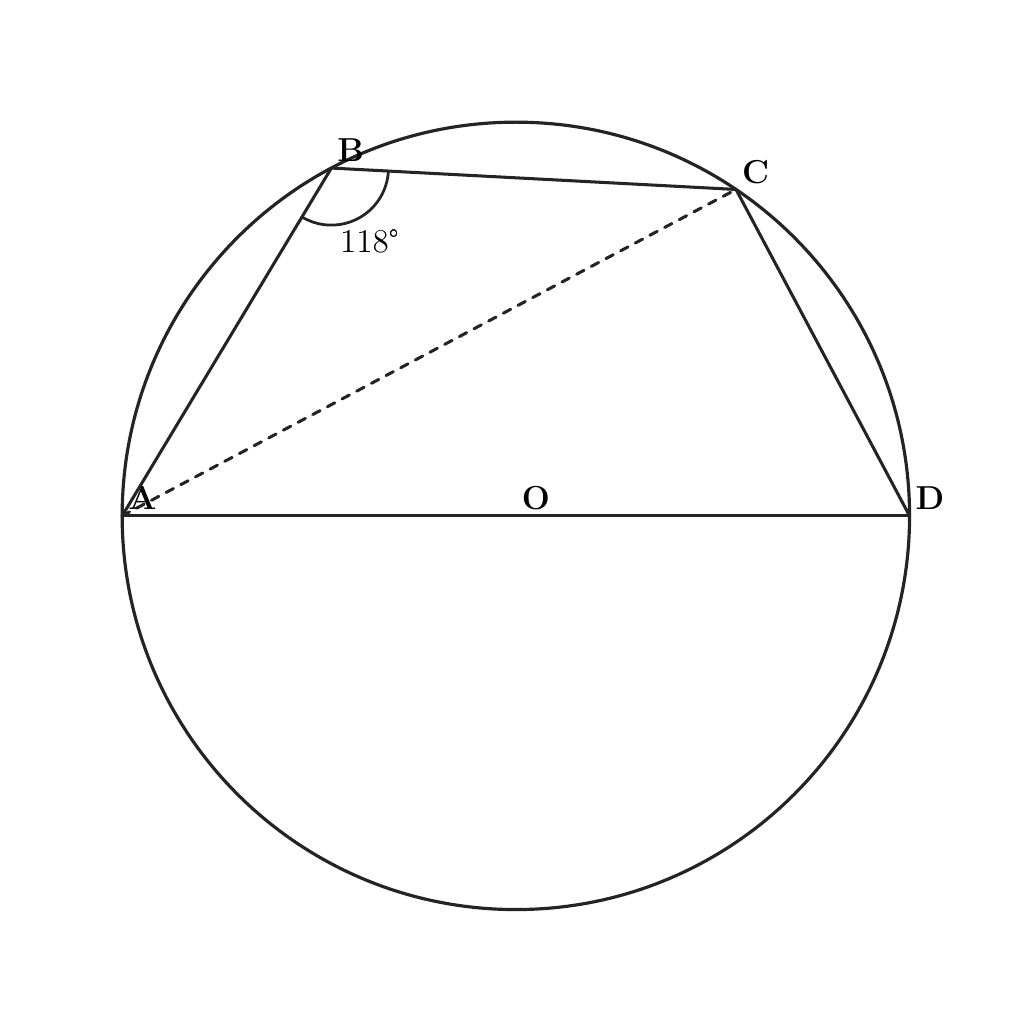
\begin{tikzpicture}[x=1.0000cm,y=1cm,line cap=round,line join=round]
\definecolor{linec0}{RGB}{35,35,40}
\definecolor{linec1}{RGB}{35,35,40}
\definecolor{linec2}{RGB}{35,35,40}
\definecolor{linec3}{RGB}{35,35,40}
\definecolor{linec4}{RGB}{35,35,40}
\definecolor{linec5}{RGB}{35,35,40}
\definecolor{edgecol}{RGB}{35,35,40}
\definecolor{hicol}{RGB}{35,35,40}
\definecolor{angcol}{RGB}{35,35,40}
\coordinate (A) at (-5.0000,0.0000);
\coordinate (B) at (-2.3429,4.4171);
\coordinate (C) at (2.7960,4.1452);
\coordinate (D) at (5.0000,0.0000);
\coordinate (O) at (0.0000,0.0000);
\draw[edgecol,line width=1.1pt] (A) -- (B);
\draw[edgecol,line width=1.1pt] (B) -- (C);
\draw[edgecol,line width=1.1pt] (C) -- (D);
\draw[edgecol,line width=1.1pt] (D) -- (A);
\draw[edgecol,line width=1.1pt,dashed] (A) -- (C);
\draw[edgecol,line width=1.15pt] (O) circle [x radius=5.0000, y radius=5.0000];
\path (-6.200,-6.200) rectangle (6.200,6.200);
\draw[edgecol,line width=1.00pt] (-2.343,4.417)++(-121.03:0.725) arc[start angle=-121.03, delta angle=118.00, radius=0.725];
\node[text=black,font=\large] at (-1.853,3.494) {118°};
\node[font=\bfseries\large,inner sep=2pt,anchor=south west] at (-5.000,0.000) {A};
\node[font=\bfseries\large,inner sep=2pt,anchor=south west] at (-2.343,4.417) {B};
\node[font=\bfseries\large,inner sep=2pt,anchor=south west] at (2.796,4.145) {C};
\node[font=\bfseries\large,inner sep=2pt,anchor=south west] at (5.000,0.000) {D};
\node[font=\bfseries\large,inner sep=2pt,anchor=south west] at (0.000,0.000) {O};
\end{tikzpicture}
\end{document}
